
This section deals with how to utilise family history and age-of-onset to increase power in a GWAS. All published methods that account for family history redefine or recalculate the phenotype. This type of improvement is different from the main focus for methodological developments so far, with methods such as BOLT-LMM\cite{loh2015efficient}, REGENIE\cite{mbatchou2021computationally}, and GATE\cite{dey2022efficient} that account for cryptic relatedness in the genotypes. The research into accounting for family history by refining the phenotype has been very limited in comparison. This is likely due to the relatively low occurrence of family history information in conjunction with genotype data. There have been some biobanks, such as UK biobank\cite{bycroft2018uk}, deCODE\cite{noauthor_2012-jh}, iPSYCH\cite{bybjerg2020ipsych2015,pedersen2018ipsych2012}, and FinnGen\cite{Kurki2022-pt}, where some level of family history information have been linked with genotypes. 

The first method we will introduce that accounts for family history is genome-wide association study by proxy (GWAX)\cite{gwax}. GWAX is not a model based approach, but rather a heuristic way to account for family history. Next, we will present the liability threshold model originally introduced by Falconer\cite{falconer1965inheritance} and extensions of this model. We will present two extensions, the first is called liability threshold model conditional on family history (LT-FH)\cite{hujoel2020liability} and the second is called LT-FH++. LT-FH++ has been developed and implemented during this PhD. As a result, it is the method this dissertation is focused on. LT-FH++ is an extension of the LT-FH method that is also able to account for age-of-onset or age, sex, and cohort effects in each included individual, while being very computationally efficient. 

\subsection{GWAX}
% GWAX
The first method that accounts for family history information is called GWAX. The method was developed and applied for Alzheimer's disease in UK biobank\cite{gwax}. It managed to increase power for a phenotype that had a low prevalence in the UK biobank participants, but was present and had a higher prevalence among their parents due to the late age-of-onset of Alzheimer's disease. GWAX is a heuristic method, i.e.\ not set in a statistical model, and the method only utilises family history and no age- or sex-related information. The GWAX phenotype is a binary variable. It considers close relatives as well when assigning case status, instead of only assigning case status based on the UK biobank participant themselves. This means an individual without Alzheimer's disease, but with a parent who did have Alzheimer's disease would be considered a case under GWAX. This approach is simple and easy to use, acts as a drop-in replacement for any previous binary phenotype, and achieved the desired result of increasing power in a GWAS setting. In short, GWAX was a big success and a proof of concept for other family history methods. There have been model based developments in family history methods since GWAX was published. The family history methods are based on the LTM, and we will therefore present it and explain how it was expanded.


\subsection{The Liability Threshold Model}
The LTM is widely used to explain how binary phenotypes can have complex aetiologies and do not behave as a Mendelian disease. Under the liability threshold model an individual will have a latent variable (a liability), $ \ell \sim N(0,1)$. The case-control status $ z $ for a given phenotype is given by 

\begin{align*}
z = 
\begin{cases}
1 & \ell \geq T \\
0 & \text{otherwise}
\end{cases},
\end{align*}
\begin{wrapfigure}{O}{7cm}
	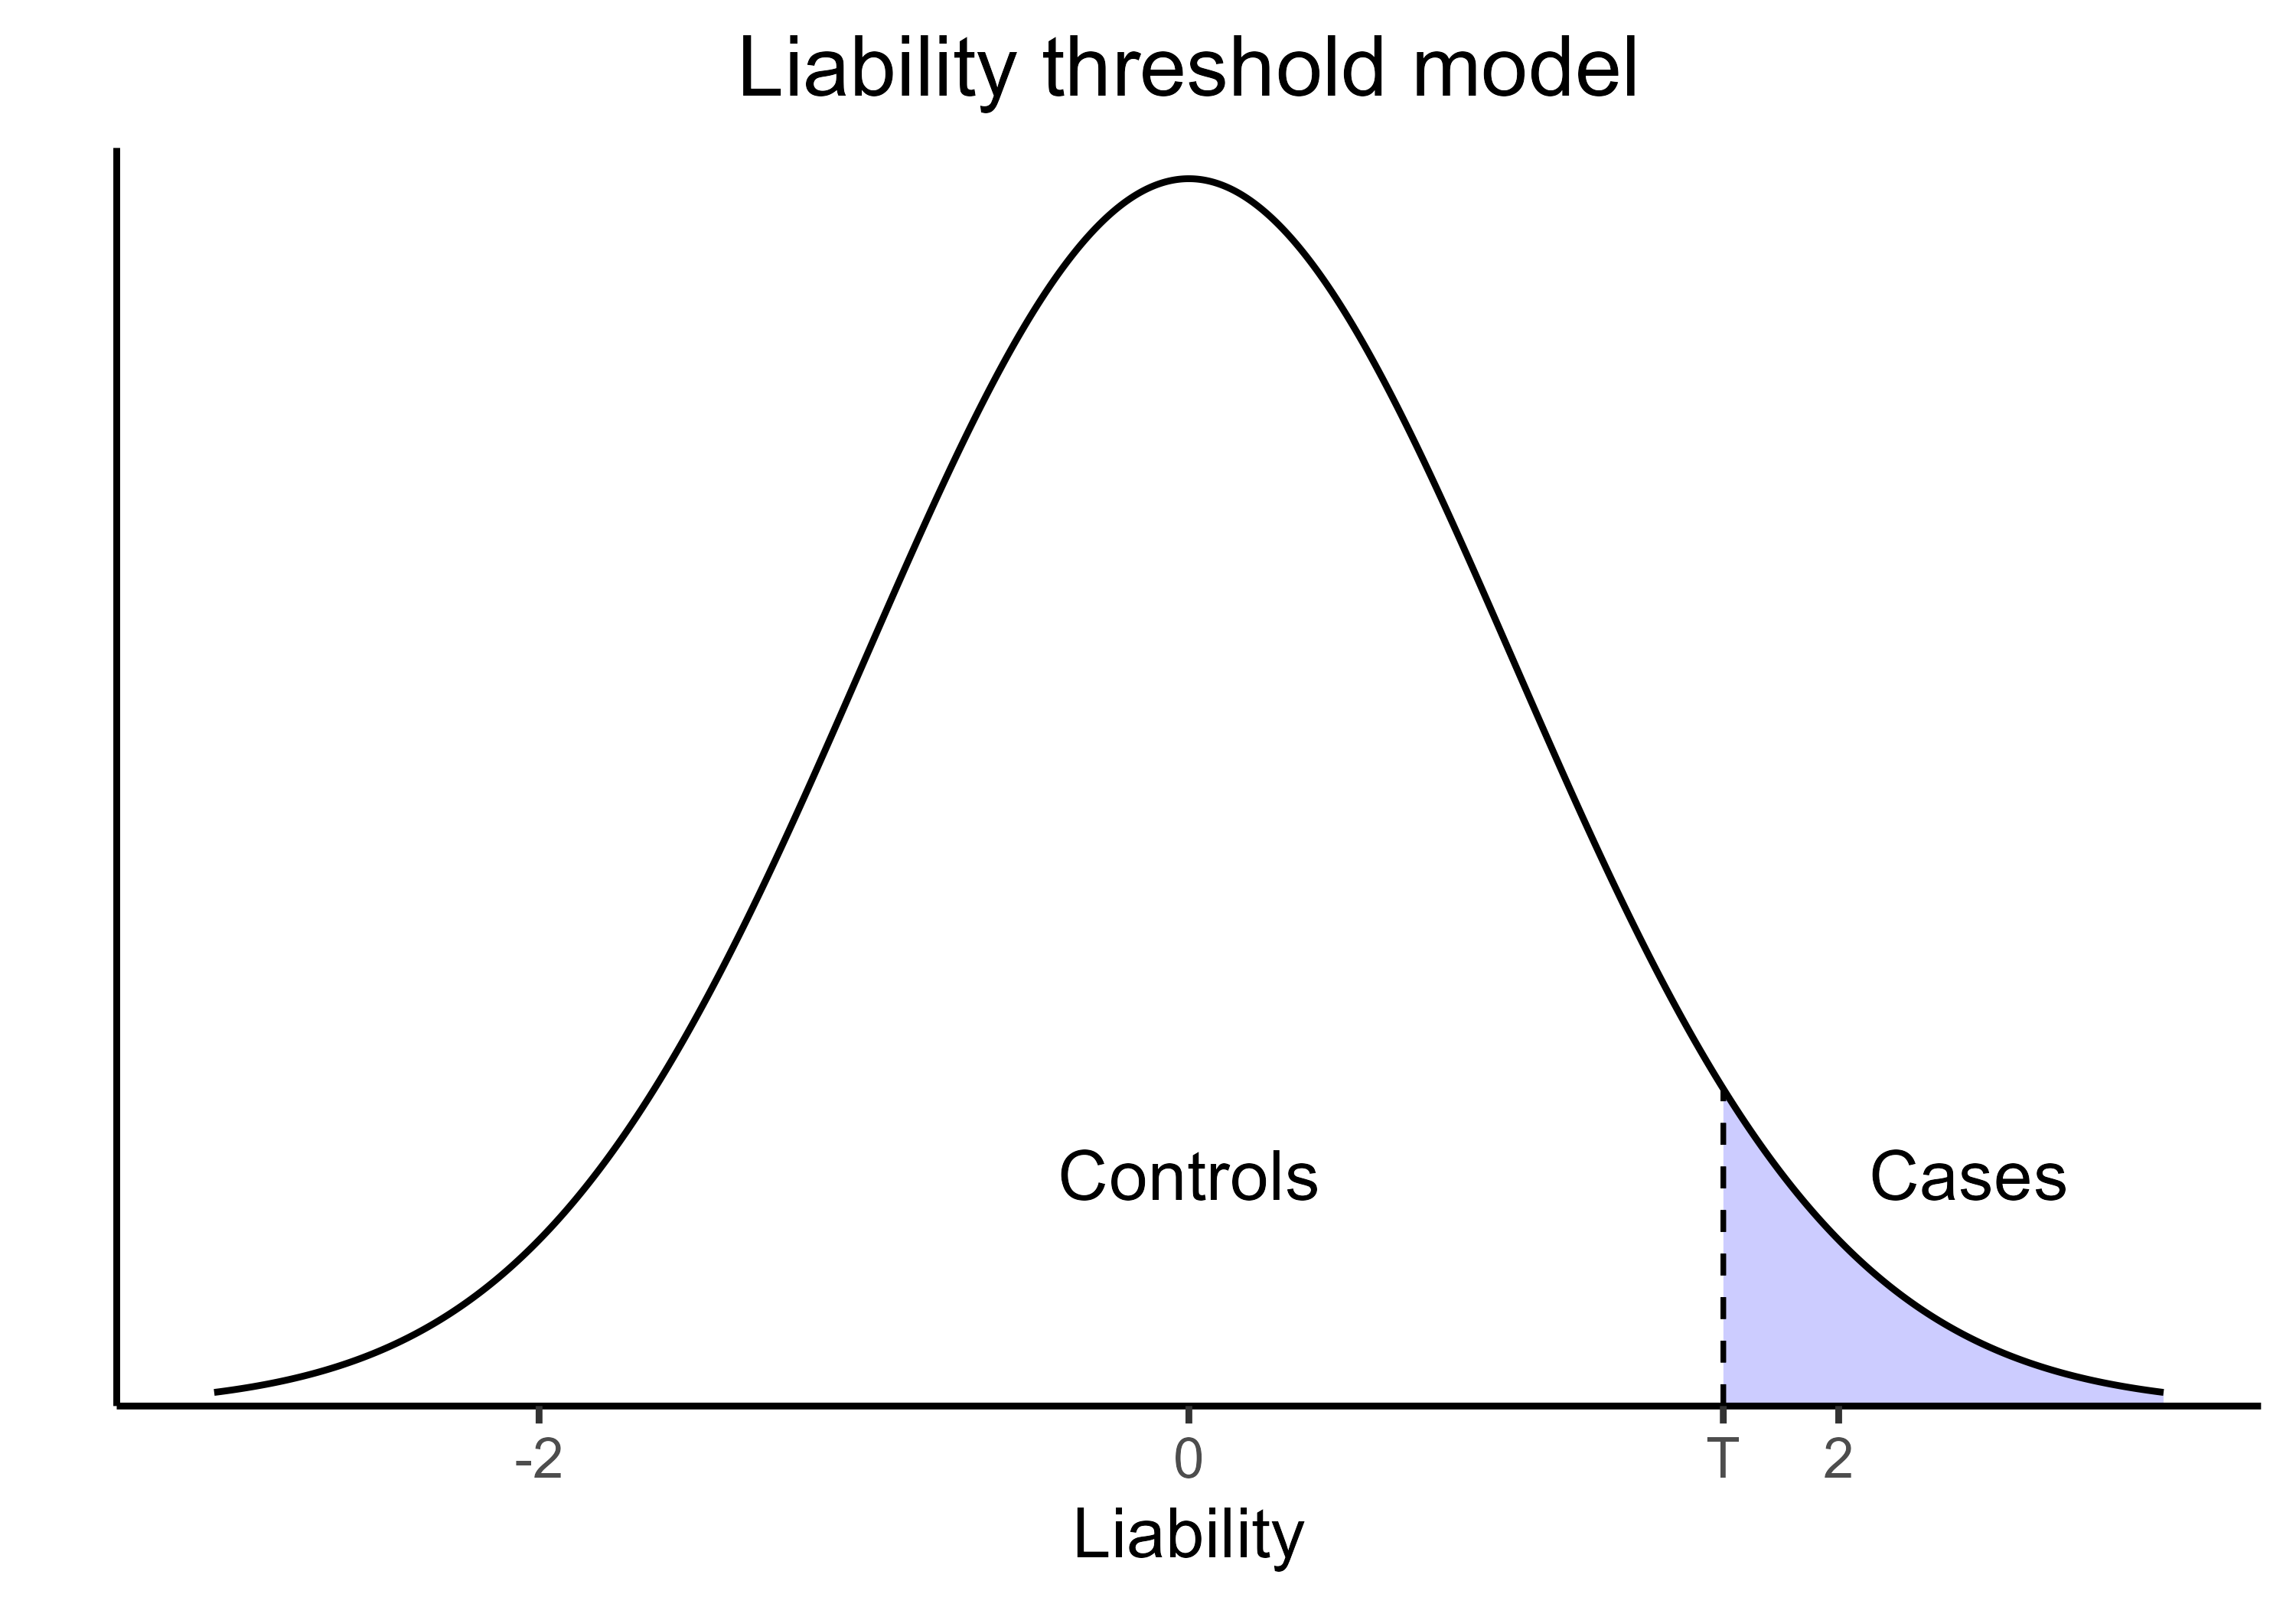
\includegraphics[width=7cm]{methods/LTM.png}
	\oldcaption{\sl Illustration of the classical liability threshold model. Liabilities above the threshold $ T $, correspond to a case diagnosis, while liabilities below $ T $ are controls.}
	\label{fig:methods:LTMplot}
\end{wrapfigure}
i.e.\ an individual is a case when the liability $ \ell $ is above a given threshold $ T $ and the threshold is determined by the prevalence $ k $, such that $ \p(\ell > T) = k $ in the population. An illustration of the LTM is provided in \cref{fig:methods:LTMplot}.

The LTM allows for modelling of non-Mendelian diseases, since the latent liability can be the result of more complex mechanisms than Mendelian diseases, which may depend on more than one or two genes \cite{falconer1967inheritance,falconer1965inheritance}. 


% LT-FH
\subsection{LT-FH}
The extension proposed by Hujoel et al.\cite{hujoel2020liability} is called LT-FH. It allows for a dependency between the genetic liability of the family members and the index person. There is no theoretical limitation on the family members to include in the model, however the original implementation only allows for both parents, the number of siblings, and a binary variable of whether any sibling has the phenotype being analysed. This is unfortunately a limitation of the data available to the authors when LT-FH was developed. In UKBB, sibling information is limited and it is only coded as present or not in any of the siblings, so we do not know which sibling(s) are affected. 

\subsubsection{The Model}

The first part of the extension is to split the full liability $ \ell_o $ in a genetic component $ \ell_g \sim N(0,h^2) $, where $ h^2 $ denotes the heritability of the phenotype on the liability scale, and an environmental component $ \ell_e \sim N(0, 1-h^2) $. Then, $ \ell_o = \ell_g + \ell_e \sim N(0,1) $ and the genetic and environmental components are independent. Others have also proposed this split into genetic and environmental components, however not with family history as well \cite{weissbrod2015accurate}. The second extension is to consider a multivariate normal distribution instead of a univariate one. For illustrative purposes, we will only show the model for which both parents are present, but no siblings. 

\begin{align}\label{eq:LTFH_model}
\ell = \left( \ell_g, \ell_o, \ell_{p_1}, \ell_{p_2} \right) \sim N(\mathbf{0}, \Sigma)^T & & &\Sigma = \begin{bmatrix}
h^2	&	h^2	&	0.5h^2	&	0.5h^2	\\
h^2 &	h^2 &	0.5h^2	&	0.5h^2	\\
0.5h^2	&	0.5h^2	&	1	&	0	\\
0.5h^2	&	0.5h^2	&	0	&	1	\\
\end{bmatrix}
\end{align}
LT-FH does not distinguish between mother and father and the parents are coded as $ p_1 $ and $ p_2 $. If available, siblings can be included in the model as well by extending the dimension of the multivariate normal distribution with the number of siblings to include. Siblings would also have a variance of $ 1 $ and a covariance of $ 0.5h^2 $ with the other family members, reflecting the liability scale heritability of the phenotype and the expected genetic overlap. If siblings are included and one is a case, then the genetic liability will be estimated under the assumption of \textit{at least one sibling is a case}. Meaning, the genetic liability is estimated for one case, two cases, etc. among the siblings, and the final estimate is a weighted average of these genetic liabilities.

\subsubsection{Input}

With this framework, the expected genetic liability can be estimated given the family member's case-control status. Estimating the expected genetic liability $ \hat{\ell_g} $ means estimating 

\begin{align*}
\hat{\ell_g} = \e \left[ \ell_g | \mathbf{Z} \right] & & & \mathbf{Z} = \left(z_o, z_{p_1}, z_{p_2} \right)^T
\end{align*}
where $ \mathbf{Z} $ is the vector of the considered family member's case-control status. The condition on $ \mathbf{Z} $ in the LTM means the liabilities for each family member is restricted to an interval. For a case, the full liability would be restricted to $ (T, \infty) $, while the full liability of a control would be restricted to $ (-\infty, T) $. If we let $ i $ indicate a given family member, e.g.\ $ o, p_1, p_2 $ and $ n $ denotes the size of the family under consideration, then the possible liabilities for a family of all cases can be described as $ \{ \ell \in \mathbb{R}^n | \ell_i \geq T_i \text{ for all } i\} $. If instead a family of all controls was considered, it would be $ \{ \ell \in \mathbb{R}^n | \ell_i < T_i \text{ for all } i\} $. The genetic liability of the index person is always unrestricted. Commonly, the area of interest would be some combination of the two sets. The restrictions on the liabilities leads to a truncated multivariate normal distribution, and calculating the expected genetic liability $ \hat{\ell_g} $ does not have an analytical solution. See \textbf{Sampling Strategy} for details on how LT-FH estimates the genetic liabilities. 

A practical consideration for LT-FH is the choice of thresholds. LT-FH considers two thresholds, one for the parents, $ T_p $, and one for the children, $ T_c $. The thresholds should reflect the prevalence for these groups, and a common strategy is to use the in-sample prevalences from UKBB. The in-sample prevalences work well enough for LT-FH in UKBB for a few reasons. First, the UKBB has a large sample size. Second, it has not been sampled for any specific phenotypes (even though they are healthier than the general population). Lastly, the LT-FH model is very robust to misspecification of its parameters.

\subsubsection{Sampling Strategy}

The sampling strategy used in the original implementation of LT-FH consists in sampling a large number of observations from the multivariate normal distribution, then splitting the samples into each of the possible configurations of $ \mathbf{Z} $, and calculate the $ \hat{\ell_g} $ by averaging within each group. More observations are sampled if the standard error of mean (sem) is larger than $ 0.1 $ in any of the configurations of $ \mathbf{Z} $. If we consider only the index person, then we will have only $ 2 $ configurations to estimate the genetic liability in and it will essentially be a rescaled case-control phenotype. If we consider the index person and one parent, we will have $ 4 $ configurations, and with two parents, there are $ 6 $ configurations, since the sex of the parent is not considered. Once siblings are considered, the max number of siblings will be considered as well as status. For up to $ 10 $ siblings and no parents, there will be $ 40 $ unique configurations. From here it scales by counting the number of siblings present, if any siblings are cases, and the parental status. A pseudocode overview of the sampling strategy can be found in Algorithm \ref{alg:LTFH}.

If a given configuration does not have an estimate of $ \hat{\ell_g} $ with sem$(\hat{\ell_g}) < 0.1 $, some resampling will be performed. This resampling is slightly more targeted than the initial sampling. For illustrative purposes, consider resampling from the configuration where one or two parents are a case, i.e.\ $ z_{p_1}  = 1$ and/or $ z_{p_2} = 1$, then univariate samples will be drawn from a truncated normal distribution on $ (T_p, \infty) $ for a case and $ (-\infty, T_p) $ for a control. Then the full model given in \cref{eq:LTFH_model} is conditioned on the targeted parental liabilities and the mean and covariance matrix in a conditional normal distribution are calculated and denoted by $ \mu^{\ast} $ and $ \Sigma^{\ast} $, respectively. Notably, not all observations from the lower dimensional conditional normal distribution are guaranteed to be observations for the desired configuration. The resampling strategy is applied until $ \hat{\ell_g} $ has a sem below $ 0.1 $ in all configurations.

\begin{algorithm}[h] 
\begin{algorithmic}[1] 
\INPUT $ h^2,$  $n_{sib},$  $\mathbf{Z},$  $T_p,$  $T_c$ 
\OUTPUT $ \hat{\ell_g} $ for all configurations
\STATE sample $ \ell \sim N(\mathbf{0}, \Sigma) $ 
\STATE split into disjoint sets from $ \mathbf{Z} $
\STATE calculate $ \hat{\ell_g} $ in each configuration 
\WHILE{sem$(\hat{\ell_g}) \geq 0.1 $ for any configuration}
	\IF{$ z_{p_1} = 1 \text{ or } z_{p_2} = 1$}
		\STATE sample  $ \ell \given \left(z_{p_1}, z_{p_2} \right)^T \sim N_{n-2}(\mu^{\ast}, \Sigma^{\ast}) $
	\ELSIF{$ z_o = 1 \text{ or } z_\mathbf{s} \neq \mathbf{0} $} 
		\STATE sample $ \ell \given \left(z_{o}, z_{\mathbf{s}} \right)^T \sim N_{n-(n_{sib} - 1)}(\mu^{\ast}, \Sigma^{\ast}) $
	\ENDIF	
	\STATE update $ \hat{\ell_g} $
\ENDWHILE
\end{algorithmic}
\caption{LT-FH sampling strategy}
\label{alg:LTFH}
\end{algorithm}


\subsection{LT-FH++}

The model underlying LT-FH and LT-FH++ is fundamentally the same, however LT-FH++ does make a few modifications to account for age-of-onset or, sex, and cohort effects. The addition of this extra information allows for a more fine-tuned estimate of the genetic liability $ \hat{\ell_g} $, further improving the genetic liability estimates. The modifications that allow for the additional information has an impact on the input and choice of sampling strategy. Therefore, this section will primarily focus on how these key points differ from LT-FH, since the fundamental model is the same, it will not be repeated. 

\subsubsection{The Model}

The model underlying LT-FH++ is very similar to LT-FH and does not differ in a major way from what is shown in eq. \ref{eq:LTFH_model}. The model used by LT-FH++ deviates from the one used in LT-FH in the family members that can be accounted for, and what information is used for each family member. In short, LT-FH considers the index person and siblings the same, since the same threshold, $ T_c $, is used for each of the children in LT-FH, and the parents are also treated the same and share the threshold $ T_p $. LT-FH++ allows for each individual to have their own personalised threshold $ T_i $, for all $ i $ in the family. The individual thresholds are based on population representative cumulative incidence proportions (CIPs). The CIPs have the interpretation of \textit{"being the proportion of individuals born in year $ y $ that have experienced a phenotype before age $ t $"}. We let $ s_i $ denote the sex of individual $ i $, which means $ k(t; s_i, b_i) $ is the CIP for individual $ i $'s sex born in year $ b_i $ at time $ t $.

\begin{align*}
\p\left( \ell_i > T_i \right) = k(t; s_i, b_i) \Rightarrow T_i = \Phi^{-1} \left(1 - k(t; s_i, b_i) \right),
\end{align*}
where $ \Phi $ denotes the CDF of the standard normal distribution. An individual's current age for control or age-of-onset for cases, their sex, and birth year will be accounted for through the choice of threshold and denoted by $ T_i $. The threshold are determined through the CIPs, which means the thresholds are also a function of $ t $, but unless it is an important distinction to make that notation will be suppressed. See \cref{sec:CIPs} for details on the CIPs. If the CIPs are stratified by birth year and sex, a more accurate estimate of an individual's full liability is provided. When age-of-onset is available for a case, their full liability can be fixed to $ T_i $, rather than spanning the interval $ (T_i, \infty) $. Furthermore, for controls the threshold will decrease as the population ages, which narrows the potential liabilities, since they have lived through a period of risk. This means that older controls will have a lower estimated liability. An illustration of how the personalised thresholds can be used in the ADuLT model see \cref{fig:adult_connection_to_CIPs}.

\begin{figure}[h]
	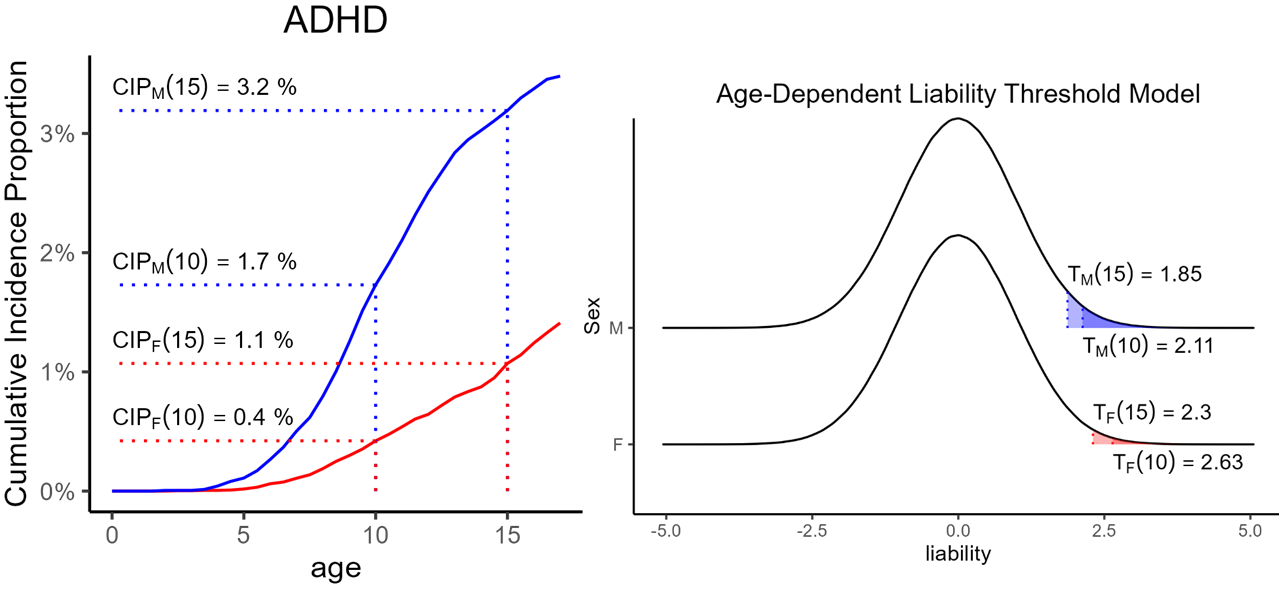
\includegraphics[width=\textwidth]{methods/adult_top.png}
	\caption[Age-dependent liability threshold model and its relationship to the CIPs]{
		\sl An illustration of how the population representative CIPs are used by the age-dependent liability threshold model. The CIPs are stratified by sex and birth year (here ADHD for individuals born in Denmark in $ 2000 $) are converted to a threshold for the ADuLT model. Females are represented by the red line, while males are represented by the blue line. The CIPs has been marked at the age of 10 and 15 for both sexes (dotted lines).}
	\label{fig:adult_connection_to_CIPs}
\end{figure}

\subsubsection{Input}
The input for LT-FH++ is similar to the input for LT-FH, but with two notable differences. The first difference is that LT-FH++ relies on CIPs for the threshold for each individual, while LT-FH utilises a general but separate threshold for parents and offspring. The second notable difference is that each family member will have to be included separately, while LT-FH does not distinguish between mother and father and only requires the total number of siblings and whether any siblings are cases. An overview of LT-FH++ and the information it is able to account for is provided in \cref{fig:LTFHppFigure1}. The sex and birth year stratified CIPs are used to assign thresholds to each individual in a family. Each person will therefore have a lower $ T_i^l $ and upper $ T_i^u $ threshold, which leads to an interval of possible liabilities defined as $ I_i = (T_i^l, T_i^u) $. For controls, the interval will be $ I_i = (T_i^l,T_i^u) = (-\infty, T_i) $, while for cases $ I_i = (T_i^l,T_i^u) = [T_i,T_i] $. If a user does not have CIPs that are stratified by sex and birth year, then a case's interval should be given as $ I_i = (T_i, \infty) $. When the thresholds have been assigned, the intervals that the truncated multivariate normal distribution have been defined and the genetic liability can be estimated. 

\begin{wrapfigure}{O}{10cm}
	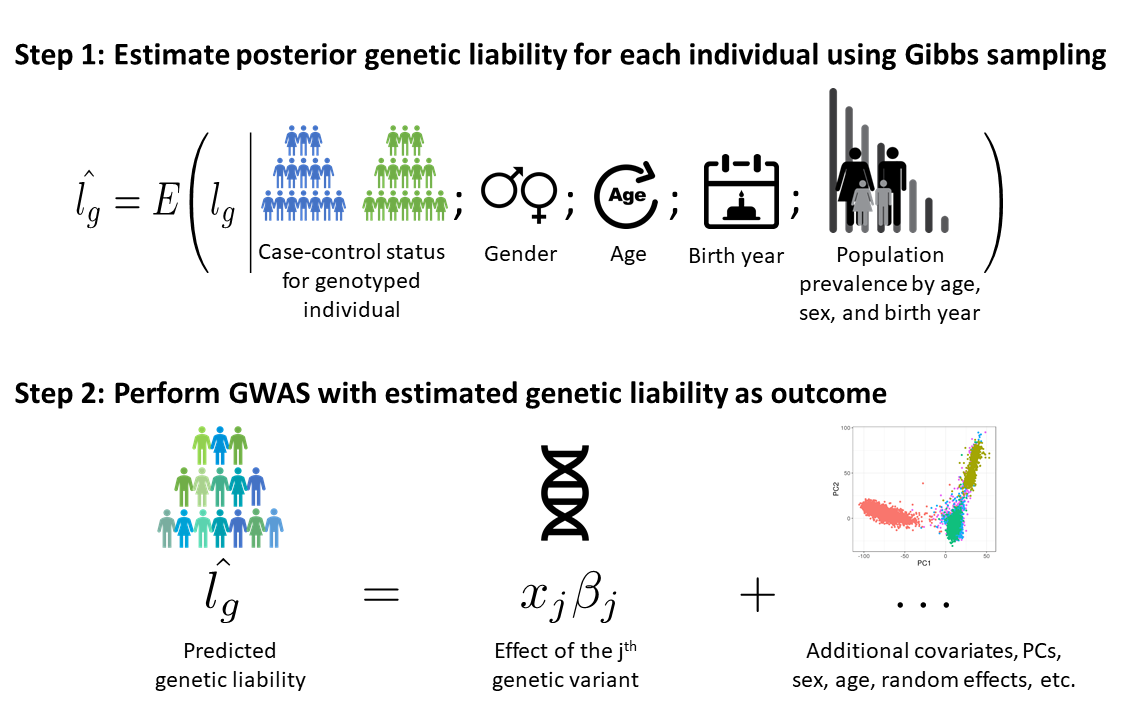
\includegraphics[width=10cm]{methods/ltfhpp_steps.png}
	%	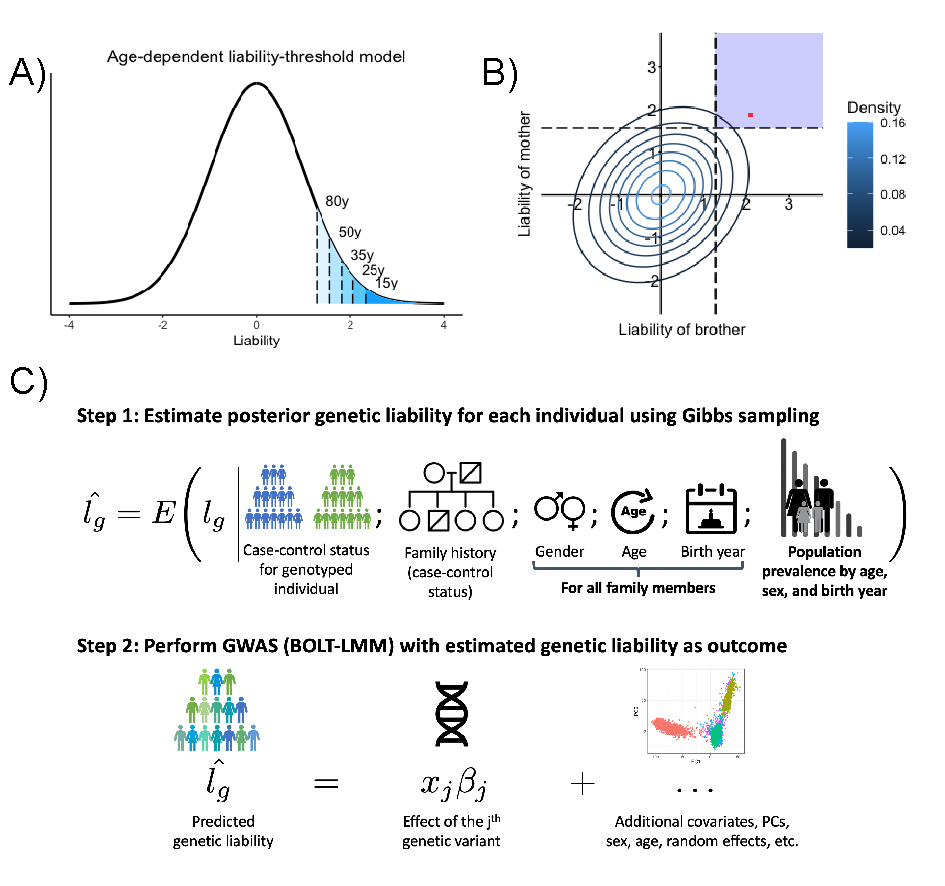
\includegraphics[width=10cm]{methods/LTFHpp_Figure1.pdf}
	\caption[Overview of LT-FH++ and what information it can account for in GWAS]{
		\sl This plot is taken as-is from the original LT-FH++ paper\cite{pedersen2022accounting}. Using LT-FH++ is a two step approach. First, a genetic liability is estimated based on the available family history, where age-of-onset or age for controls, sex, and birth year is accounted for in each included individual. Then a GWAS can be performed with the GWAS software of choice, e.g.\ BOLT-LMM.
	} % Esben said it was fine to include this plot as is.
	\label{fig:LTFHppFigure1}
\end{wrapfigure}

\subsubsection{Sampling Strategy}

Due to the unlikeliness that two families will consist of the exact same sex, age-of-onset, etc., and fixing the upper and lower limit for cases, the truncated normal distributions will be unique to each family. The straight-forward sampling approach employed by LT-FH is therefore not computationally tractable any more. Instead LT-FH++ employs a Gibbs sampler to sample directly from a truncated multivariate normal distribution with predefined limits. To further improve the computational complexity of LT-FH++, we have used a slightly modified version of the Gibbs sampler approach suggested by the \textit{tmvtnorm} R package\cite{wilhelm2015gibbs,wilhelm2010tmvtnorm}. Pseudo code of the Gibbs sampler used by LT-FH++ is presented in \cref{alg:LTFH++}.

% pseudo code for the Gibbs sampler

\begin{algorithm}
\begin{algorithmic}[1]
\INPUT $ h^2,$ $T_{i}^l,$ $T_{i}^u$ and each family member's role 
\OUTPUT $ \hat{\ell_g} $ for all index persons
\GIBBS
\STATE \textbf{Initialise} $\ell^{(0)}$ as $ \mathbf{0} $ and pre-compute $ \Sigma_{12} \Sigma_{22}^{-1} $ and $ \Sigma_{12} \Sigma_{22}^{-1} \Sigma_{21} $ for $ \mu_i^{(s)} $ and $ \sigma^2_i $
\FOR{$ s = 1, \ldots, S$}
	\FOR{$ j = 1, \ldots, n+1 $}  \COMMENT{n+1 is family size + genetic liability}
	%% should include uniform draw transformed to possible range of liabilities
	\STATE $ U \sim \text{Unif}(I_i) = \text{Unif}(T_i^l, T_i^u) $ \COMMENT{Ensures truncation}
	\STATE $ \ell_j^{(s)} = F^{-1}_{N(\mu_i^{(s)}, \sigma_i^2)}(U) $
%	$\ell_j^{(s)} \sim N(\mu_i^{(s)}, \sigma_i^2)$
	\ENDFOR
\ENDFOR
\IF{sem$(\hat{\ell_g}) \geq 0.1 $}
\STATE rerun Gibbs Sampler
\ELSE
\STATE return  $ \hat{\ell_g} $
\ENDIF
\end{algorithmic}
\caption{LT-FH++ sampling strategy}
\label{alg:LTFH++}
\end{algorithm}


\subsection{LT-FH++ with Correlated Traits} \label{sec:methods:ltfhpp:correlatedTraits}
LT-FH++ can be extended to include correlated traits. Many disorder pairs have a non-zero genetic correlation, which is often not used. There exist methods that can account for correlated traits, with the most popular method being MTAG\cite{turley2018multi}. However, MTAG requires a GWAS to be run on each of the correlated phenotypes and can then account for some of the genetic signal between the phenotype's summary statistics. Both MTAG and LT-FH++ can account for multiple correlated phenotypes at a time. LT-FH++ deals with correlated traits by using the additional traits to further refine the liability estimate of the primary phenotype, while MTAG uses summary statistics to correct for each other's effect. This means a single GWAS is performed with a LT-FH++ phenotype that accounts for case-control status and family history of the correlated phenotype(s), rather than separate GWASs being run for each phenotype. 

If two phenotypes are genetically correlated, the LT-FH++ model can account for the correlated phenotype by extending the covariance matrix. The simplest way to account for correlated phenotypes requires the same information as a single trait analysis, so stratified CIPs and family history for each phenotype, as well as the genetic correlation of the considered phenotypes. The thresholds will be determined within each phenotype with the disorder specific CIPs.

If we consider $ \ell_1 $ and $ \ell_2 $ as the vectors of liabilities for some family for two genetically correlated disorders, each of the vectors can be modelled as seen above for a single trait. However, the interaction between the two disorders would be ignored. Setting $ h_1^2 $ and $ h_2^2 $ to be the liability-scale heritability for the two disorders and setting $ \Sigma^{(1)} $ and $ \Sigma^{(2)} $ to be the covariance matrices for the two genetically correlated disorders, we can model the interaction with the following model

\begin{equation*}
	\ell = \left(\ell_1, \ell_2\right)^T \sim N(\mathbf{0}, \Sigma), \quad \Sigma = 
	\begin{pmatrix} 
		\Sigma^{(1)} & \Sigma^{(12)} \\
		\Sigma^{(21)} & \Sigma^{(2)} 
	\end{pmatrix}, \quad \Sigma^{(12)}_{ij} = K_{ij}\rho_{12}\sqrt{h_1^2 h_2^2},
\end{equation*}
where $ \Sigma_{ij}^{(12)} $ is the expected genetic overlap between two individuals and genetic covariance between the disorders, expressed by the genetic correlation $ \rho_{12} $ and the heritabilities. We can generalise the construction of the covariance matrix such that it can be used to create the between-disorder covariance as well as the with-in disorder covariance matrix for the considered family. First, let $ K_{ij} $ denote the expected genetic overlap between individuals $ i $ and $ j $, let $ \rho_{nm} $ be the genetic correlation between phenotype $ n $ and $ m $. If we only consider one phenotype, then $ \rho_{nn} = 1$. Then we can construct the covariance matrix entry-wise with 

\begin{equation*}
	\Sigma^{(nm)}_{ij} = K_{ij} \rho_{nm}\sqrt{h^2_{n}h^2_{m}}, \qquad K_{ij} = 
	\begin{cases} 
		1 		& \text{if } i \text{ and } j \text{ the same} \\
		0.5 	& \text{if } i \text{ and } j \text{ $1^{st}$ degree} \\
		0.25 	& \text{if } i \text{ and } j \text{ $2^{nd}$ degree} \\ 
		0.125 	& \text{if } i \text{ and } j \text{ $3^{rd}$ degree}  \\
		0 		& \text{otherwise}
	\end{cases}.
\end{equation*}
With this construction, it is also possible to readily extend the considered family members to a broader pedigree. The considered pedigrees in the LT-FH and the LT-FH++ papers only allowed for first degree relatives. This limitation has been loosened, and far broader pedigrees can now be used. The extensions to the possible family members were made while developing the correlated trait implementation. The correlated trait and extended family were intended to be used in the fGRS paper\textbf{TODO: proper reference}. The extended family means we can account for family history in children of the index person, paternal and maternal grandparents, half-siblings, aunts, and uncles can also be considered. Considering the extended family and correlated traits both serve the purpose of further refining the liability estimate.

There are not changes to the sampling strategy, as the Gibbs sampler proposed is scalable to many dimensions.
